\documentclass{ximera}


\graphicspath{
  {./}
  {ximeraTutorial/}
  {basicPhilosophy/}
}

\newcommand{\mooculus}{\textsf{\textbf{MOOC}\textnormal{\textsf{ULUS}}}}

\usepackage{tkz-euclide}\usepackage{tikz}
\usepackage{tikz-cd}
\usetikzlibrary{arrows}
\tikzset{>=stealth,commutative diagrams/.cd,
  arrow style=tikz,diagrams={>=stealth}} %% cool arrow head
\tikzset{shorten <>/.style={ shorten >=#1, shorten <=#1 } } %% allows shorter vectors

\usetikzlibrary{backgrounds} %% for boxes around graphs
\usetikzlibrary{shapes,positioning}  %% Clouds and stars
\usetikzlibrary{matrix} %% for matrix
\usepgfplotslibrary{polar} %% for polar plots
\usepgfplotslibrary{fillbetween} %% to shade area between curves in TikZ
\usetkzobj{all}
\usepackage[makeroom]{cancel} %% for strike outs
%\usepackage{mathtools} %% for pretty underbrace % Breaks Ximera
%\usepackage{multicol}
\usepackage{pgffor} %% required for integral for loops



%% http://tex.stackexchange.com/questions/66490/drawing-a-tikz-arc-specifying-the-center
%% Draws beach ball
\tikzset{pics/carc/.style args={#1:#2:#3}{code={\draw[pic actions] (#1:#3) arc(#1:#2:#3);}}}



\usepackage{array}
\setlength{\extrarowheight}{+.1cm}
\newdimen\digitwidth
\settowidth\digitwidth{9}
\def\divrule#1#2{
\noalign{\moveright#1\digitwidth
\vbox{\hrule width#2\digitwidth}}}






\DeclareMathOperator{\arccot}{arccot}
\DeclareMathOperator{\arcsec}{arcsec}
\DeclareMathOperator{\arccsc}{arccsc}

















%%This is to help with formatting on future title pages.
\newenvironment{sectionOutcomes}{}{}


\author{Lee Wayand}

\begin{document}
\begin{exercise}  





Below is the graph of $y=N(m)$.  

\begin{image}
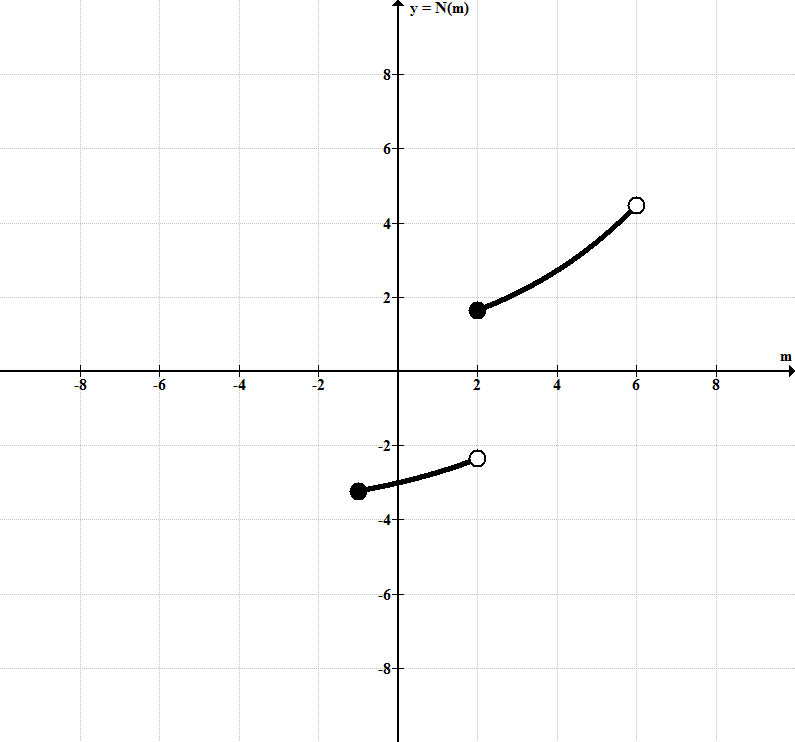
\includegraphics{../../func_graphs/f6.png}
\end{image}









\begin{question} 


What is the domain of $N$?\\


\begin{multipleChoice}
\choice {$[-1, 6]$}
\choice [correct]{$[-1, 6)$}
\choice {$[-1, 2) \cup  (2, 6)$}
\choice {$[-1, 2) \cup  (2, 6]$}
\end{multipleChoice}

\end{question}






\begin{question} 


What is the range of $g$?\\


\begin{multipleChoice}
\choice {$[-3.2, 4.5]$}
\choice {$[-3.2, 4.5)$}
\choice [correct]{$[-3.2, -2.2) \cup  [1.8, 4.5)$}
\choice {$[-1, 2) \cup  (2, 6)$}
\end{multipleChoice}


\end{question}









\begin{question} 



\[  N(2) = \answer[tolerance=0.25]{1.8}  \]

\end{question}










\begin{question} 



$N(m)$ is an increasing function.
\begin{multipleChoice}
\choice [correct]{True}
\choice {False}
\end{multipleChoice}

\end{question}









\begin{question} 



The minimum of $N(m)$ is $\answer[tolerance=0.25]{-3.2}$.   \\

The maximum of $N(m)$ is $\answer{DNE}$.
 

\end{question}






\begin{question} 


The minimum of $N(m)$ occurs at $\answer[tolerance=0.25]{-1}$.   

\end{question}









\end{exercise}
\end{document}